\documentclass[a4paper,10pt]{article}

\usepackage[a4paper, left=2.0cm, right=2.0cm, top=2.0cm, bottom=2.0cm]{geometry}
\usepackage[T1]{fontenc}
\usepackage{newtxtext,newtxmath}
\usepackage{amsmath}
\usepackage{graphicx}
\usepackage{booktabs}
\usepackage{array}

\newcolumntype{P}[1]{>{\raggedright\arraybackslash}p{#1}}

% Metric names (set in text font to match the surrounding prose)
\newcommand{\PushRatio}{\textrm{push\_ratio}}
\newcommand{\Spread}{\textrm{spread}}
\newcommand{\Push}{\textrm{push}}

\title{
Evaluating the Detectability of Malicious Updates in Federated Learning\\[0.8em]
\large
--- Along the Axes of Data Heterogeneity and Attack Stealthiness ---
}
\author{3CDA2216 Shusei Kasahara}
\date{\today}

% Abstract (placed below the title)
\makeatletter
\g@addto@macro\@maketitle{%
  \begin{center}
  \begin{minipage}{0.9\textwidth}
  \small
  \textbf{Abstract}\quad
  In Federated Learning (FL), the global model can be poisoned by updates sent from malicious clients. In this study, we treat the detection of malicious updates as a binary classification of the update vectors just before aggregation, and evaluate the detection performance of four detectors with ROC-AUC while varying the degree of data heterogeneity (Non-IID degree) and the stealthiness of the attack. The results show that the ranking of the detectors switched depending on the attack, and that the degradation of detection performance under Non-IID data corresponded not to the magnitude of the dispersion of benign updates but to how that dispersion was distributed. Moreover, because high-dimensional benign updates lie at an almost constant distance from their mean, malicious updates close to the mean were in fact conspicuous. These results do not support the central hypothesis that detectability is largely determined by the ratio between the push of malicious updates and the dispersion of benign updates; instead, they suggest that detectability depends on where malicious updates are located in the quantity each detector looks at, and on the shape of the distribution of benign updates.
  \par\vspace{0.5em}
  \textbf{Keywords:}\quad Federated Learning $\cdot$ Model Poisoning Attack $\cdot$ Malicious Update Detection $\cdot$ Non-IID
  \end{minipage}
  \end{center}
  \vspace{0.5em}%
}
\makeatother

\begin{document}

\maketitle

\section{Introduction}

Federated Learning (FL) is a distributed learning framework in which multiple clients collaboratively train a model without sharing raw data\cite{mammen2021fl}. However, FL faces the threat of Model Poisoning Attacks, in which malicious clients tamper with model updates\cite{sagar2023survey}. In particular, stealthy attacks such as ALIE\cite{baruch2019little}, which keep malicious updates within the range of the dispersion of benign updates, can evade even Robust Aggregation.

The contest between attack and defense takes place in the space of update vectors just before the server performs aggregation in each round. In this study, we therefore regard defense as a binary classification problem of distinguishing malicious updates from benign ones, and evaluate the detection performance of four detectors by ROC-AUC on the update vectors, separately from the final accuracy.

Most prior studies evaluate the effect of defenses by final accuracy or attack success rate. Li et al.\ (2023)\cite{li2023experimental} compared attacks including ALIE under both IID and Non-IID settings and showed that robustness drops considerably under Non-IID data, but their evaluation was based on final accuracy. In contrast, the novelty of this study lies in the following three points.
\begin{itemize}
  \item We evaluate how distinguishable malicious updates are, round by round during training, using ROC-AUC on the update vectors just before aggregation.
  \item We simultaneously vary two factors, the degree of data heterogeneity (Non-IID degree) and the stealthiness of the attack, and investigate the conditions under which detection breaks down.
  \item We attempt to explain the degradation of detection performance under Non-IID data in terms of the ratio between the push of malicious updates and the dispersion of benign updates (push\_ratio), as well as the shape of the distribution of benign updates.
\end{itemize}

The results of this study suggest that detectability is not largely determined by \PushRatio{}, but depends on where malicious updates lie in the quantity each detector looks at, and on the shape of the distribution of benign updates.

\section{Related Work}

Sagar et al.\ conducted a comprehensive survey of poisoning attacks and defenses in FL. They classify attacks into Data Poisoning Attacks and Model Poisoning Attacks, and systematically organize defenses from viewpoints such as Robust Aggregation and anomaly detection\cite{sagar2023survey}.

Fang et al.\ proposed Local Model Poisoning Attacks against Byzantine-robust FL. By formulating the attack as an optimization problem, they realized attacks that are effective even against Byzantine-robust aggregation methods such as Krum, Bulyan, Median, and Trimmed Mean, showing that existing defenses are insufficient\cite{fang2020local}.

Foundations of Robust Aggregation include Krum by Blanchard et al.\cite{blanchard2017krum}, coordinate-wise Median/Trimmed Mean by Yin et al.\cite{yin2018byzantine}, and Bulyan by El Mhamdi et al.\cite{elmhamdi2018hidden}. These provide theoretical guarantees against up to a certain fraction of Byzantine clients, but all implicitly assume that ``benign updates are close to each other,'' and the guarantees weaken in Non-IID environments.

Baruch et al.\ proposed the ``A Little Is Enough'' (ALIE) attack, in which all malicious clients collude to send a small perturbation that stays within the coordinate-wise standard deviation of benign updates, and showed that it can evade Trimmed Mean, Krum, and Bulyan\cite{baruch2019little}. Shejwalkar et al.\ proposed aggregation-agnostic min-max/min-sum attacks and a detection method based on singular value decomposition (Divide-and-Conquer)\cite{shejwalkar2021manipulating}.

Detection-based defenses include FLAME\cite{nguyen2022flame}, which combines clustering on cosine distance with weight clipping.

For handling data heterogeneity, label partitioning with the Dirichlet distribution by Hsu et al.\cite{hsu2019measuring} is standard, and NIID-Bench\cite{li2022federated} systematically compares various partitioning schemes.

Two prior studies are particularly close to this work. Li et al.\ (2023) conducted an experimental study comparing eight Robust Aggregation methods and five Byzantine attacks (including ALIE) on FedSGD/FedAvg under both IID and Non-IID settings, and showed that the robustness of all methods drops considerably on Non-IID data, with some degrading even in the absence of malicious clients\cite{li2023experimental}. However, their evaluation metric was final accuracy, and they did not address how robustness changes during training. Wang et al.\ showed that similarity measures such as cosine similarity, $L_2$ norm, and Euclidean distance have the weakness that, in high-dimensional parameter spaces, they may judge updates as similar even when the parameter values differ substantially, and proposed an attack, Faker, that exploits this weakness\cite{wang2023trust}. This result indicates that detectors based on cosine distance (corresponding to D2 in this study) can be deceived by attacks.

Most of these studies either evaluate by final accuracy or attack success rate, or report detection performance only at a single Non-IID level. Note that this study does not propose a new attack optimized for Non-IID environments; rather, it analyzes the relationship between detection performance and the dispersion of benign updates.

\section{Research Questions and Hypothesis}
\label{sec:rq}

\subsection{Research Questions}

This study addresses the following three questions. First, to what extent can malicious updates in FL be distinguished by anomaly detection at the level of update vectors, and how does detection performance differ among representative aggregation-agnostic detectors? Second, how does the degree of data heterogeneity (Non-IID degree) degrade detection performance, and can that degradation be explained by an increase in the dispersion of benign updates? Third, how does the stealthiness of the attack, i.e., the degree to which malicious updates are kept within the benign cluster, affect detection performance, and where is the boundary at which detection breaks down?

\subsection{Central Hypothesis}

\begin{quote}
Whether malicious updates are detectable is largely determined by whether the push of the malicious updates exceeds the dispersion among benign clients. Since Non-IID data increases the dispersion of benign updates, it lets attacks blend into the benign diversity and degrades detection performance.
\end{quote}

As explanatory variables for testing this hypothesis, we introduce the spread of the benign cluster \Spread{}, the push distance of malicious updates \Push{}, and their ratio \PushRatio{} (defined in Section~\ref{sec:metrics}). If the hypothesis is correct, we should observe that detection performance (ROC-AUC) drops sharply in the region where \PushRatio{} falls below $1$, and that the stronger the Non-IID degree, the smaller \PushRatio{} becomes for the same attack strength. However, for ALIE (A2), \PushRatio{} is by construction almost equal to $z$ and does not change with the Non-IID degree (Section~\ref{sec:attacks}). Therefore, the observed relationship between \PushRatio{} and AUC is examined with the sign-flipping attack (A1), while A2 is used as a condition in which \PushRatio{} is moved above and below $1$ via $z$, and as a condition in which only the Non-IID degree is varied while \PushRatio{} is held constant.

\section{Threat Model}
\label{sec:threat}

In this study, we assume the following threat model for the attacker and the defender. The attacker is assumed to have full knowledge; that is, malicious clients can observe the updates of benign clients in each round and can collude with each other. In our experiments, this attacker is simulated on the server side. The set of malicious clients is fixed throughout all rounds; its fraction is assumed to satisfy $f/n \le 0.3$, and we use $f/n = 0.2$ in the experiments.

The defender resides on the server and can observe the update vectors of all clients, but has no clean data. Hence, defenses such as FLTrust\cite{cao2021fltrust}, in which the server holds a small amount of clean data and uses it as the basis of trust, are out of scope. The ground-truth labels indicating which clients are malicious are used only for evaluation and are never given to the detectors.

This threat model is an optimistic setting favorable to the attacker. Shejwalkar et al.\cite{shejwalkar2022back} argue that the threat of poisoning is limited under realistic constraints, but this study is positioned as evaluating ``the upper bound of detection performance.''

\section{Evaluation Framework}
\label{sec:framework}

\subsection{Notation}

In communication round $t$, let the model update vector of participating client $i \in \{1,\dots,n\}$ be $g_i = w_i - w_{\text{global}}$. Let $B$ be the index set of benign clients and $M$ the index set of malicious clients ($|M| = f$), and let $\bar{g}_B = \frac{1}{|B|}\sum_{i \in B} g_i$ be the mean of benign updates. FedAvg\cite{mcmahan2017fedavg} is used for aggregation: in every round, the updates of all clients are averaged with weights proportional to each client's data size.

\subsection{Detectors}
\label{sec:detectors}

We use four general-purpose detectors D1--D4 that do not depend on the aggregation method. Each detector assigns an anomaly score $s_i$ (larger means more likely malicious) to each client $i$.

\paragraph{D1: Norm deviation}
\begin{equation}
s_i = \left|\; \|g_i\|_2 - \operatorname*{median}_{j}\|g_j\|_2 \;\right|
\end{equation}
With an even number of clients, the scores of the two clients straddling the median are equal by definition, so they are treated as ties regardless of numerical error. D1 is the simplest detector; it is effective against attacks that substantially change the norm (scaling or random noise) but is expected to be weak against stealthy attacks. It corresponds to weight-clipping defenses such as FLAME\cite{nguyen2022flame}.

\paragraph{D2: Cosine distance to a reference direction}
Using the coordinate-wise median $r = \operatorname{median}(g_1,\dots,g_n)$ as the reference direction,
\begin{equation}
s_i = 1 - \frac{g_i \cdot r}{\|g_i\|_2\,\|r\|_2}.
\end{equation}
D2 captures anomalies in the direction of updates and corresponds to the idea of FLAME\cite{nguyen2022flame}.

\paragraph{D3: Two-cluster clustering}
We use four features $\phi_i$ for each update: the norm $\|g_i\|_2$, the D2 score, and the projections onto the first and second principal components. After standardizing each feature, we apply $k$-means ($k=2$), regard the larger cluster as benign, and use the distance to its centroid as the score. All pairs of points are tried as initial centers, and the partition with the smallest within-cluster sum of squares is adopted. This corresponds to the idea of Auror\cite{shen2016auror}.

\paragraph{D4: Spectral residual}
We compute the first right singular vector $v$ of the matrix $\tilde{G} = [\tilde{g}_1;\dots;\tilde{g}_n]$ formed by stacking the centered updates $\tilde{g}_i = g_i - \frac{1}{n}\sum_{k=1}^{n} g_k$, and set
\begin{equation}
s_i = (\tilde{g}_i \cdot v)^2 .
\end{equation}
D4 corresponds to the ideas of Spectral Signatures\cite{tran2018spectral} and Divide-and-Conquer\cite{shejwalkar2021manipulating}.

\subsection{Attacks}
\label{sec:attacks}

\paragraph{A1: Sign-flipping attack}
\begin{equation}
g_i^{\text{mal}} = -\,g_i \qquad (i \in M)
\end{equation}
Each malicious client flips the sign of the update $g_i$ obtained by honest training on its own local data and sends it. Its direction is exactly opposite to that of its own benign update, while its norm is unchanged. A1 is a crude attack that direction-based detectors should detect easily, and is used as a baseline.

\paragraph{A2: ALIE}
We use the update generation rule of ALIE (A Little Is Enough) proposed by Baruch et al.\cite{baruch2019little}. The attacker computes the coordinate-wise mean $\mu$ and standard deviation $\sigma$ from the benign clients' updates in the current round, and sets
\begin{equation}
g_i^{\text{mal}} = \mu - z\,\sigma \qquad (i \in M);
\label{eq:alie}
\end{equation}
all malicious clients send this identical vector. While the original paper estimates $\mu$ and $\sigma$ from the malicious workers' own data, this study computes them from the benign clients' updates themselves, assuming a stronger attacker than in the original paper.

We use eight levels of $z$: $0.385$, $0.5$, $0.75$, $1$, $1.25$, $1.5$, $2$, and $3$. The smallest value, $0.385$, is the upper bound of the perturbation $z_{\max}$ defined in the original paper under a normality assumption, applied to our setting of $n=20,\ f=4$; it is used as a reference value, not as a theoretical upper bound in Non-IID environments. The original paper also uses $z$ larger than $z_{\max}$, e.g., $z=1.5$ on MNIST. Note that ``undetected'' in the original paper means not being excluded by Trimmed Mean and being selected by Krum; it does not mean being indistinguishable from benign updates as whole update vectors. Moreover, since benign updates in Non-IID environments do not necessarily satisfy the distributional assumptions of the original paper, this study does not assume the theoretical guarantees of ALIE, but applies the same generation rule to different Non-IID conditions and compares detection performance.

For ALIE, \PushRatio{} (Section~\ref{sec:metrics}) is almost determined by construction. Since $\mu$ equals the benign mean $\bar{g}_B$, taking $\sigma$ to be the population standard deviation and letting $d_i = \|g_i - \bar{g}_B\|_2$, we have
\begin{equation}
\PushRatio
= z \cdot \frac{\sqrt{\frac{1}{|B|}\sum_{i \in B} d_i^2}}{\frac{1}{|B|}\sum_{i \in B} d_i}
\;\ge\; z .
\label{eq:alie-pushratio}
\end{equation}
That is, for A2 with fixed $z$, \PushRatio{} stays almost constant even across conditions with different Non-IID degrees.

\subsection{Data Distribution (Non-IID)}
\label{sec:data-noniid}

We use label partitioning based on the Dirichlet distribution\cite{hsu2019measuring}. For each client $k$, class proportions $q_k \sim \mathrm{Dir}(\alpha \pi)$ are drawn, and every client receives the same amount of data ($1{,}500$ samples) according to those proportions, where $\pi$ is the class proportion of the entire training set. A larger $\alpha$ brings every client's proportions closer to $\pi$ (IID), whereas a smaller $\alpha$ skews the classes each client holds. We use three levels, $\alpha \in \{1000\;(\approx\text{IID}),\; 5,\; 1\}$. The fraction of the most frequent class held by a client, averaged over 10 trials, is $12\%,\ 38\%,\ 65\%$ for $\alpha=1000,\ 5,\ 1$, respectively. The total amount of distributed data is $30{,}000$ samples, half of the $60{,}000$ training samples, and each client uses 80\% of its data ($1{,}200$ samples) for local training.

Non-IID data comes in several types, such as label distribution skew, feature distribution skew, and quantity skew\cite{li2022federated}. The ``Non-IID degree'' in this study refers only to label distribution skew. We equalized the data size across all clients because unequal data sizes would change update norms and FedAvg weights, making it impossible to attribute changes in detection performance to label distribution skew.

\subsection{Detection Performance Metric}
\label{sec:roc-auc}

An anomaly detector assigns each sample an anomaly score $s$ (larger means more anomalous). The trajectory of the pair of false positive rate and true positive rate $(\mathrm{FPR}, \mathrm{TPR})$ as the threshold moves from $+\infty$ to $-\infty$ is called the ROC curve, and the area under it is called ROC-AUC (hereafter AUC)\cite{fawcett2006roc}. AUC has the following probabilistic interpretation\cite{hanley1982meaning}. Letting $M$ be the set of malicious (positive) samples and $B$ the set of benign (negative) samples,
\begin{equation}
\mathrm{AUC}
= \frac{1}{|M|\,|B|}\sum_{i \in M}\sum_{j \in B}
\Bigl( \mathbf{1}[s_i > s_j] + \tfrac{1}{2}\,\mathbf{1}[s_i = s_j] \Bigr),
\label{eq:auc}
\end{equation}
which equals ``the probability that the score of a randomly chosen malicious sample exceeds that of a randomly chosen benign sample.'' $\mathrm{AUC}=1$ indicates perfect separation, $\mathrm{AUC}=0.5$ is equivalent to random ranking, and $\mathrm{AUC}<0.5$ means that the detector judges malicious samples to be ``more benign'' than benign ones. Because AUC does not depend on the choice of threshold and is relatively insensitive to the class ratio even in imbalanced settings where malicious samples are a minority, it is suitable for evaluating whether a detector separates malicious from benign samples.

\subsection{Evaluation Metrics}
\label{sec:metrics}

In each round $t$, we obtain pairs of anomaly score and malicious label $(s_i, y_i)$ for all clients ($y_i = 1$ if malicious). As the detection performance metric we use the threshold-independent ROC-AUC (defined in Section~\ref{sec:roc-auc}). AUC is computed for each round; we show its trajectory over rounds and also summarize it per condition. Since rounds within the same run are not independent, for the summary we first average the AUC over rounds 46--50 within each trial, and then compute the mean and standard deviation across trials.

As explanatory variables for testing the central hypothesis, we define the mean distance of benign updates from the benign mean \Spread{}, the mean distance of malicious updates from the benign mean \Push{}, and their ratio \PushRatio{} as follows:
\begin{align*}
  \Spread &= \tfrac{1}{|B|}\textstyle\sum_{i \in B}\|g_i - \bar{g}_B\|_2, \\
  \Push   &= \tfrac{1}{|M|}\textstyle\sum_{i \in M}\|g_i - \bar{g}_B\|_2, \\
  \PushRatio &= \Push\,/\,\Spread.
\end{align*}

The relationship between \PushRatio{} and AUC is evaluated for the sign-flipping attack using Spearman's rank correlation coefficient $\rho$ for each detector. Since \PushRatio{} under sign flipping varies mainly with $\alpha$, we compute the correlation for each $\alpha$ in addition to the overall correlation. Because $\rho$ does not assume a linear relationship and is robust to outliers, it is suitable for evaluating the relationship between \PushRatio{}, which varies over orders of magnitude, and AUC, which saturates at an upper bound of 1. Ties are handled by average ranks. For ALIE, we show plots of AUC against $z$ for each $\alpha$.

Furthermore, since detection difficulty may differ depending on how benign updates are spread even for the same \Spread{}, we record in each round the following two metrics representing the structure of the distribution of benign updates. These are explanatory variables for discussion that use ground-truth labels, and are not given to the detectors. First, from the singular values $\{\sqrt{\lambda_k}\}$ of the matrix of centered benign updates, we compute the explained variance ratio of the first principal component, $\lambda_1 / \sum_k \lambda_k$. This represents the degree to which benign updates are concentrated in a particular direction; we also compute the same quantity for all updates including malicious ones, which is what D4 actually uses. Second, for the angle between the malicious direction $a = \bar{g}_M - \bar{g}_B$ (where $\bar{g}_M$ is the mean of malicious updates) and the first principal component $v_1$, we compute $|\cos\theta| = |a \cdot v_1| / (\|a\|_2\,\|v_1\|_2)$, both for the first principal component of benign updates only and for that of all updates (the projection direction of D4).

\section{Experiments}
\label{sec:experiment}

\subsection{Environment and Training Settings}
\label{sec:exp-setting}

Table~\ref{tab:exp-setting} lists the training and environment settings, and Table~\ref{tab:exp-conditions} the experimental conditions. We use a small CNN following Fang et al.\cite{fang2020local}. We set the number of local epochs to 2 because each client has only $1{,}200$ training samples, and with one epoch, training did not progress sufficiently within 50 rounds. Even with this setting, however, training at $\alpha=1$ had not converged by round 50 (Section~\ref{sec:res-acc}). Since detection performance can change across rounds (Section~\ref{sec:res-rounds}), we use the values of rounds 46--50 as the representative value of each condition and also show the trajectory over rounds.

\begin{table}[t]
\centering
\begin{minipage}[t]{0.51\textwidth}
\centering
\caption{Training and environment settings}
\label{tab:exp-setting}
\small
\begin{tabular}{@{}l@{\hspace{0.8em}}P{4.3cm}@{}}
\toprule
Item & Value \\
\midrule
Dataset & MNIST (10-class classification) \\
Model & Small CNN (following Fang) \\
Number of clients $n$ & 20 (all participate every round) \\
Data per client & $1{,}500$ samples ($1{,}200$ for training) \\
Communication rounds & 50 \\
Local epochs & 2 \\
Batch size & 32 \\
Learning rate & $0.01$ \\
Optimizer & SGD (no momentum) \\
Aggregation & FedAvg \\
Implementation & PyTorch / Flower (simulation) \\
Hardware & CPU \\
\bottomrule
\end{tabular}
\end{minipage}\hfill
\begin{minipage}[t]{0.47\textwidth}
\centering
\caption{Experimental conditions}
\label{tab:exp-conditions}
\small
\begin{tabular}{@{}lP{4.6cm}@{}}
\toprule
Axis & Levels \\
\midrule
Non-IID degree $\alpha$ & $1000,\; 5,\; 1$ \\
Attack & Sign flipping (A1), ALIE (A2, $z=0.385,\ 0.5,\ 0.75,\ 1,$ $1.25,\ 1.5,\ 2,\ 3$) \\
Malicious fraction $f/n$ & $0.2$ (fixed, $f=4$) \\
Detectors & D1--D4 \\
Trials & $10$ \\
\bottomrule
\end{tabular}
\end{minipage}
\end{table}

\subsection{Experimental Conditions}
\label{sec:exp-conditions}

The attacked conditions amount to $3\,(\alpha) \times 9\,(\text{attacks}) \times 10\,(\text{trials}) = 270$ runs; in addition, we ran $30$ runs without attack to obtain baseline values of \Spread{} and accuracy ($300$ runs in total). The set of malicious clients is fixed throughout all rounds within each trial, and the trial index determines the random seeds for data partitioning, model initialization, data shuffling during local training, and the selection of malicious clients. As a result, trials with the same index have the same four malicious clients regardless of $\alpha$ and the attack.

\subsection{Implementation and Measurement}
\label{sec:exp-impl}

The experimental system was built with the simulation feature of Flower\cite{beutel2020flower}, running 20 virtual clients on a single machine. The sign-flipping attack (A1) was implemented inside the malicious clients by flipping the sign of the update obtained from training before returning it. On the server side, we extended the FedAvg strategy and inserted the following processing after all client replies had arrived and before aggregation. First, for ALIE (A2), the coordinate-wise mean and standard deviation are computed from the benign clients' updates, and the malicious clients' updates are replaced with the vector of Eq.~(\ref{eq:alie}). This simulates the threat model of Section~\ref{sec:threat} on the server side. Next, the four detectors are applied to the set of update vectors after the attack, and the scores, ROC-AUC, \Spread{}, \Push{}, \PushRatio{}, and the distribution-structure metrics are recorded for each round. The malicious labels are used only for evaluation and for computing the distribution-structure metrics, and are not given to the detectors. Finally, aggregation is performed with FedAvg without using the detection results. In addition, the test accuracy of the global model was recorded for each round.

\section{Results}
\label{sec:results}

All 300 runs (270 with attack, 30 without) completed 50 rounds as configured in Tables~\ref{tab:exp-setting} and \ref{tab:exp-conditions}. Unless otherwise stated, values in the tables below are means across trials.

\subsection{Training Convergence and the Effect of Attacks on Accuracy}
\label{sec:res-acc}

Table~\ref{tab:acc} shows the test accuracy of the global model at round 50, and Fig.~\ref{fig:acc-round} shows the accuracy over rounds.

\begin{table*}[t]
\centering
\caption{Test accuracy at round 50 [\%] (mean $\pm$ standard deviation over 10 trials) and the increase in accuracy from round 45 to round 50 [percentage points] (mean over 10 trials)}
\label{tab:acc}
\small
\begin{tabular}{@{}lcccccc@{}}
\toprule
 & \multicolumn{3}{c}{Accuracy at round 50} & \multicolumn{3}{c}{Increase over rounds 45--50} \\
\cmidrule(lr){2-4}\cmidrule(l){5-7}
Attack & $\alpha=1000$ & $\alpha=5$ & $\alpha=1$ & $\alpha=1000$ & $\alpha=5$ & $\alpha=1$ \\
\midrule
No attack & $98.02 \pm 0.11$ & $97.43 \pm 0.24$ & $94.30 \pm 1.25$ & 0.14 & 0.17 & 0.53 \\
A1 Sign flipping & $97.09 \pm 0.20$ & $95.03 \pm 1.01$ & $76.25 \pm 7.84$ & 0.16 & 0.26 & 0.05 \\
\midrule
A2 $z{=}0.385$ & $98.00 \pm 0.10$ & $97.29 \pm 0.25$ & $92.94 \pm 2.47$ & 0.13 & 0.16 & 0.63 \\
A2 $z{=}0.5$ & $97.99 \pm 0.08$ & $97.29 \pm 0.25$ & $92.89 \pm 2.50$ & 0.14 & 0.16 & 0.64 \\
A2 $z{=}0.75$ & $98.01 \pm 0.08$ & $97.29 \pm 0.26$ & $92.78 \pm 2.57$ & 0.13 & 0.17 & 0.69 \\
A2 $z{=}1$ & $98.01 \pm 0.10$ & $97.28 \pm 0.25$ & $92.63 \pm 2.69$ & 0.14 & 0.16 & 0.65 \\
A2 $z{=}1.25$ & $98.00 \pm 0.11$ & $97.27 \pm 0.25$ & $92.47 \pm 2.74$ & 0.12 & 0.16 & 0.63 \\
A2 $z{=}1.5$ & $98.00 \pm 0.11$ & $97.24 \pm 0.26$ & $92.35 \pm 2.69$ & 0.13 & 0.12 & 0.67 \\
A2 $z{=}2$ & $97.96 \pm 0.10$ & $97.19 \pm 0.26$ & $91.75 \pm 2.78$ & 0.13 & 0.14 & 0.70 \\
A2 $z{=}3$ & $97.86 \pm 0.11$ & $96.97 \pm 0.31$ & $89.11 \pm 3.28$ & 0.11 & 0.15 & 0.88 \\
\bottomrule
\end{tabular}
\end{table*}

\begin{figure*}[t]
\centering
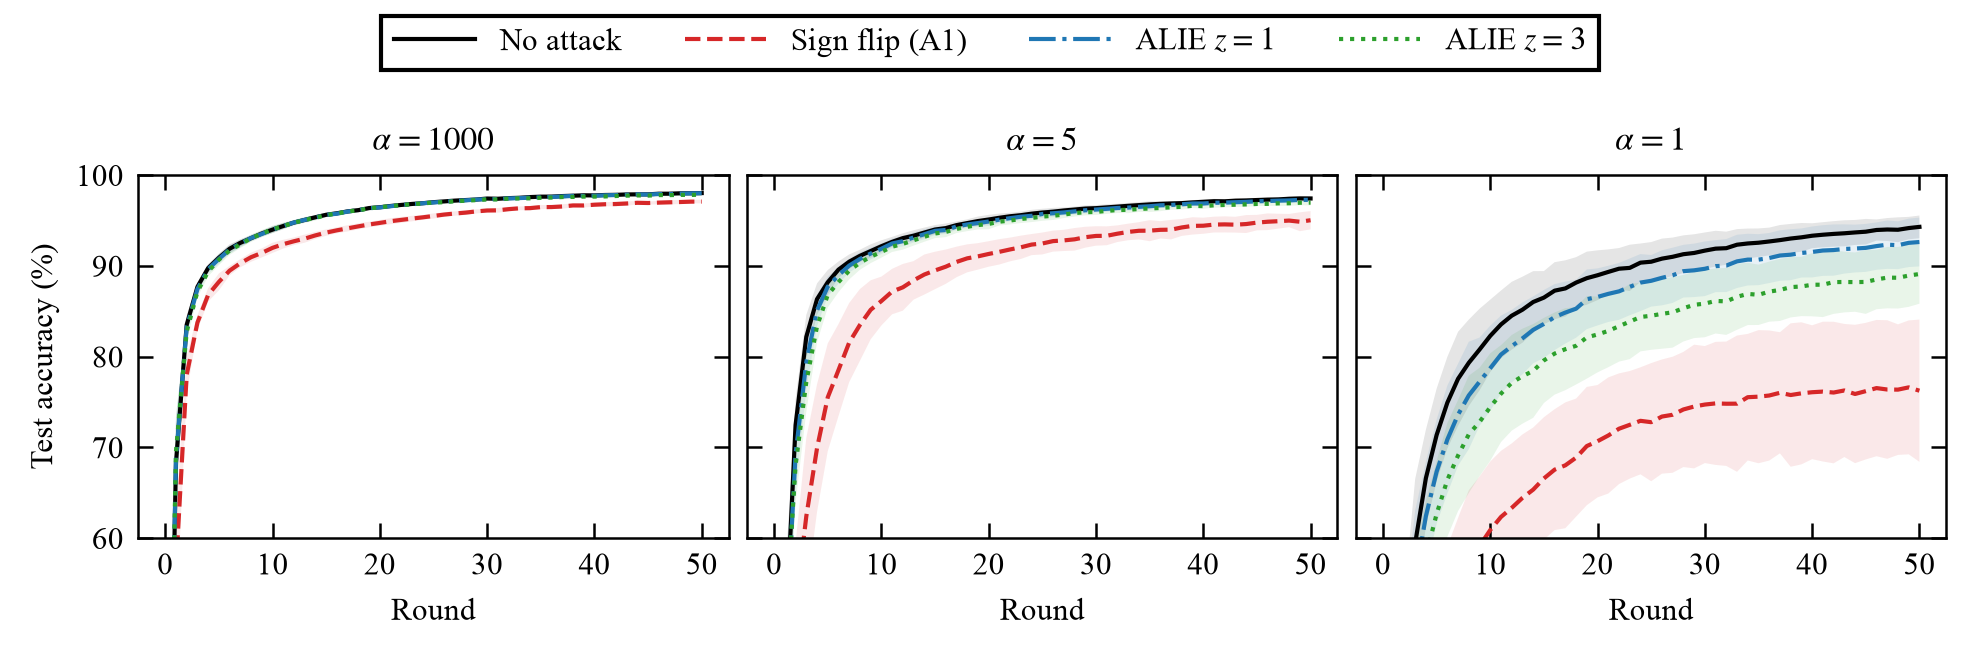
\includegraphics[width=0.75\textwidth]{fig/accuracy_by_round_v3.png}
\caption{Test accuracy over rounds (mean over 10 trials; bands show $\pm$ standard deviation). For ALIE, only $z=1$ and $z=3$ of the eight levels are shown. The vertical axis shows $60\%$ and above.}
\label{fig:acc-round}
\end{figure*}

Without attack, the accuracy was $98.0\%$, $97.4\%$, and $94.3\%$ for $\alpha=1000,\,5,\,1$, respectively. However, at $\alpha=1$ the accuracy still rose by about $0.5$ points over rounds 45--50, so the detection performance at rounds 46--50 for $\alpha=1$ reflects a stage before training had fully converged. Sign flipping reduced accuracy by about $0.9$ and $2.4$ points for $\alpha=1000$ and $5$, respectively, and by about $18$ points for $\alpha=1$. In contrast, for ALIE the difference from the no-attack condition was at most $0.5$ points for any $z$ at $\alpha=1000,\,5$, and within 2 points for $z \le 1.5$ even at $\alpha=1$.

\subsection{Overview of Detection Performance}
\label{sec:res-final}

Table~\ref{tab:final-auc} shows the ROC-AUC at rounds 46--50, and Fig.~\ref{fig:auc-z} shows the relationship between ALIE's $z$ and AUC.

\begin{table*}[t]
\centering
\caption{ROC-AUC at rounds 46--50 (mean over 10 trials after averaging rounds 46--50 within each trial; $\pm$ is shown when the standard deviation across trials is $0.10$ or larger)}
\label{tab:final-auc}
\footnotesize
\tabcolsep=3.5pt
\begin{tabular}{@{}l@{\hspace{5pt}}cccc@{\hspace{8pt}}cccc@{\hspace{8pt}}cccc@{}}
\toprule
 & \multicolumn{4}{c}{$\alpha=1000$} & \multicolumn{4}{c}{$\alpha=5$} & \multicolumn{4}{c}{$\alpha=1$} \\
\cmidrule(lr){2-5}\cmidrule(lr){6-9}\cmidrule(l){10-13}
Attack & D1 & D2 & D3 & D4 & D1 & D2 & D3 & D4 & D1 & D2 & D3 & D4 \\
\midrule
A1 Sign flipping & 0.97 & 1.00 & 1.00 & 1.00 & 0.94 & 1.00 & 0.99 & 0.97 & 0.88 & 1.00 & 0.98 & 0.85$\pm$0.12 \\
\midrule
A2 $z{=}0.385$ & 1.00 & 0.00 & 0.96 & 0.09 & 1.00 & 0.00 & 1.00 & 0.04 & 0.97 & 0.00 & 0.97 & 0.04 \\
A2 $z{=}0.5$ & 1.00 & 0.00 & 0.96 & 0.16$\pm$0.10 & 1.00 & 0.00 & 1.00 & 0.06 & 0.96 & 0.00 & 0.97 & 0.07 \\
A2 $z{=}0.75$ & 1.00 & 0.00 & 0.99 & 1.00 & 1.00 & 0.00 & 1.00 & 0.39$\pm$0.21 & 0.88$\pm$0.10 & 0.00 & 0.93$\pm$0.12 & 0.16$\pm$0.11 \\
A2 $z{=}1$ & 0.88 & 0.00 & 0.99 & 1.00 & 0.84 & 0.00 & 1.00 & 1.00 & 0.47$\pm$0.20 & 0.00 & 0.98 & 0.81$\pm$0.26 \\
A2 $z{=}1.25$ & 0.16 & 0.00 & 0.98 & 1.00 & 0.09 & 0.00 & 0.99 & 1.00 & 0.14$\pm$0.16 & 0.00 & 0.98 & 1.00 \\
A2 $z{=}1.5$ & 0.99 & 0.00 & 0.99 & 1.00 & 0.94 & 0.00 & 1.00 & 1.00 & 0.72$\pm$0.18 & 0.00 & 0.98 & 1.00 \\
A2 $z{=}2$ & 1.00 & 0.83$\pm$0.17 & 0.99 & 1.00 & 1.00 & 0.12$\pm$0.13 & 1.00 & 1.00 & 0.99 & 0.00 & 0.98 & 1.00 \\
A2 $z{=}3$ & 1.00 & 1.00 & 1.00 & 1.00 & 1.00 & 1.00 & 1.00 & 1.00 & 1.00 & 0.97 & 0.98 & 1.00 \\
\bottomrule
\end{tabular}
\end{table*}

\begin{figure*}[t]
\centering
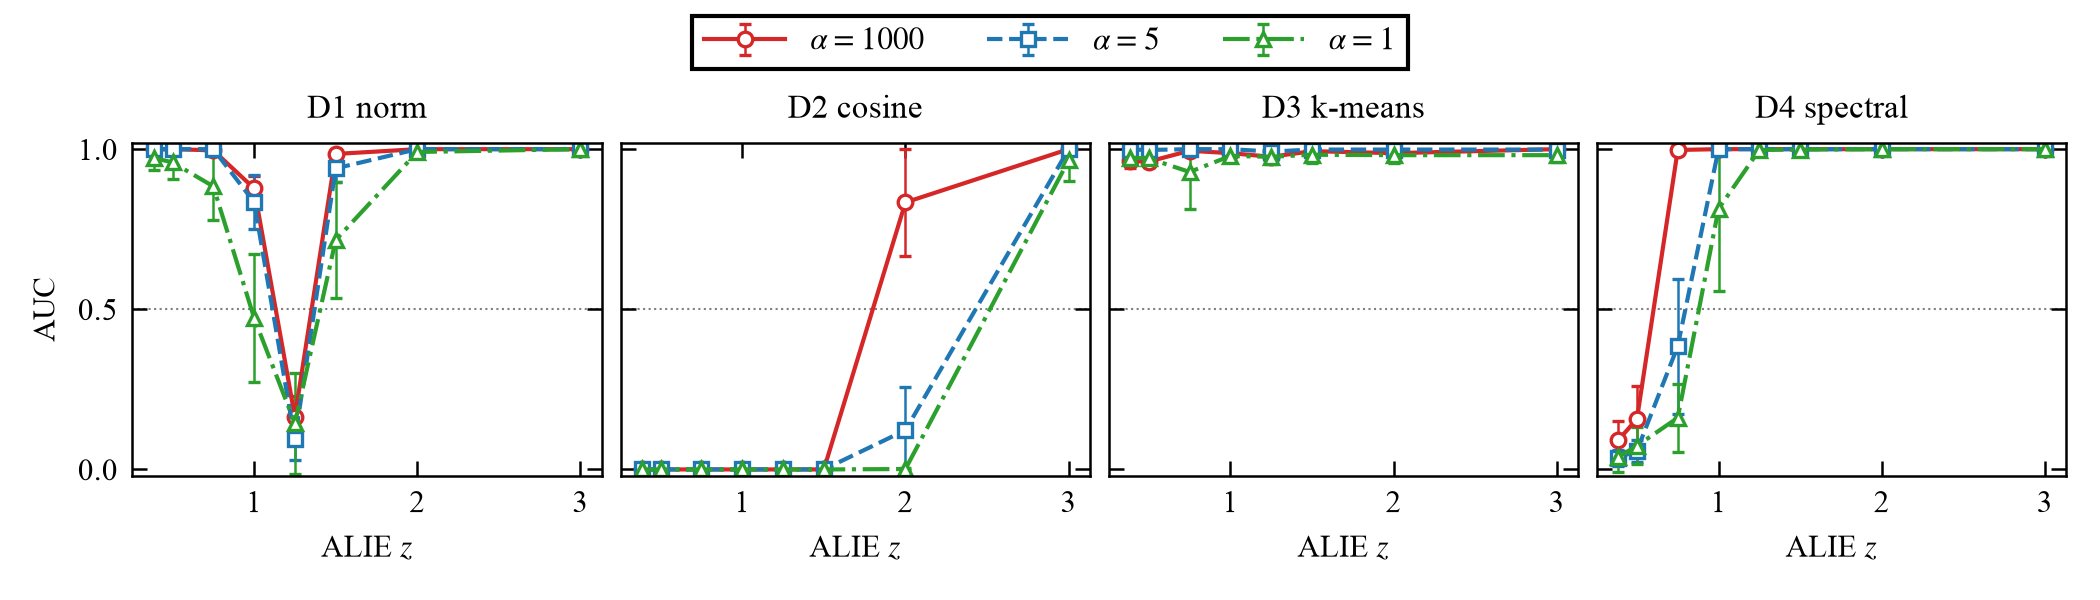
\includegraphics[width=\textwidth]{fig/detection_auc_by_z_v3.png}
\caption{ALIE's $z$ and AUC at rounds 46--50. Points are means over 10 trials; bars show $\pm$ standard deviation. Red solid line with circles: $\alpha=1000$; blue dashed line with squares: $\alpha=5$; green dash-dotted line with triangles: $\alpha=1$. The dotted line indicates $\mathrm{AUC}=0.5$.}
\label{fig:auc-z}
\end{figure*}

Against the sign-flipping attack, D2 and D3 achieved $\mathrm{AUC} \ge 0.97$ for all $\alpha$. D1 and D4 decreased as $\alpha$ decreased: for $\alpha=1000,\,5,\,1$, D1 was $0.97$, $0.94$, $0.88$ and D4 was $1.00$, $0.97$, $0.85$.

Against ALIE, D2 had an AUC of $0.00$ for all $\alpha$ when $z \le 1.5$, i.e., the ranking was completely inverted. At $z=2$, it was $0.83$, $0.12$, $0.00$ for $\alpha=1000,\,5,\,1$, and at $z=3$ it was $0.96$ or higher for all $\alpha$. D1's AUC was $0.95$ or higher for all $\alpha$ when $z \le 0.5$, reached its minimum ($0.09$--$0.16$) at $z=1.25$, and was $0.99$ or higher for all $\alpha$ when $z \ge 2$. D3 achieved $\mathrm{AUC} \ge 0.92$ under all conditions. D4 was inverted ($0.04$--$0.16$) for small $z$ and rose to nearly $1.0$ beyond a certain $z$. For $\alpha=1000$ and $5$, the switch was abrupt, occurring between $z=0.5$ and $0.75$ and between $z=0.75$ and $1$, respectively. For $\alpha=1$, it was more gradual: the AUC was $0.16$ at $z=0.75$, $0.81$ at $z=1$, and $1.00$ for $z \ge 1.25$.

\subsection{AUC over Rounds}
\label{sec:res-rounds}

Fig.~\ref{fig:auc-round} shows the AUC over rounds for each detector (mean $\pm$ standard deviation across trials). For ALIE, only four of the eight levels are shown.

\begin{figure*}[t]
\centering
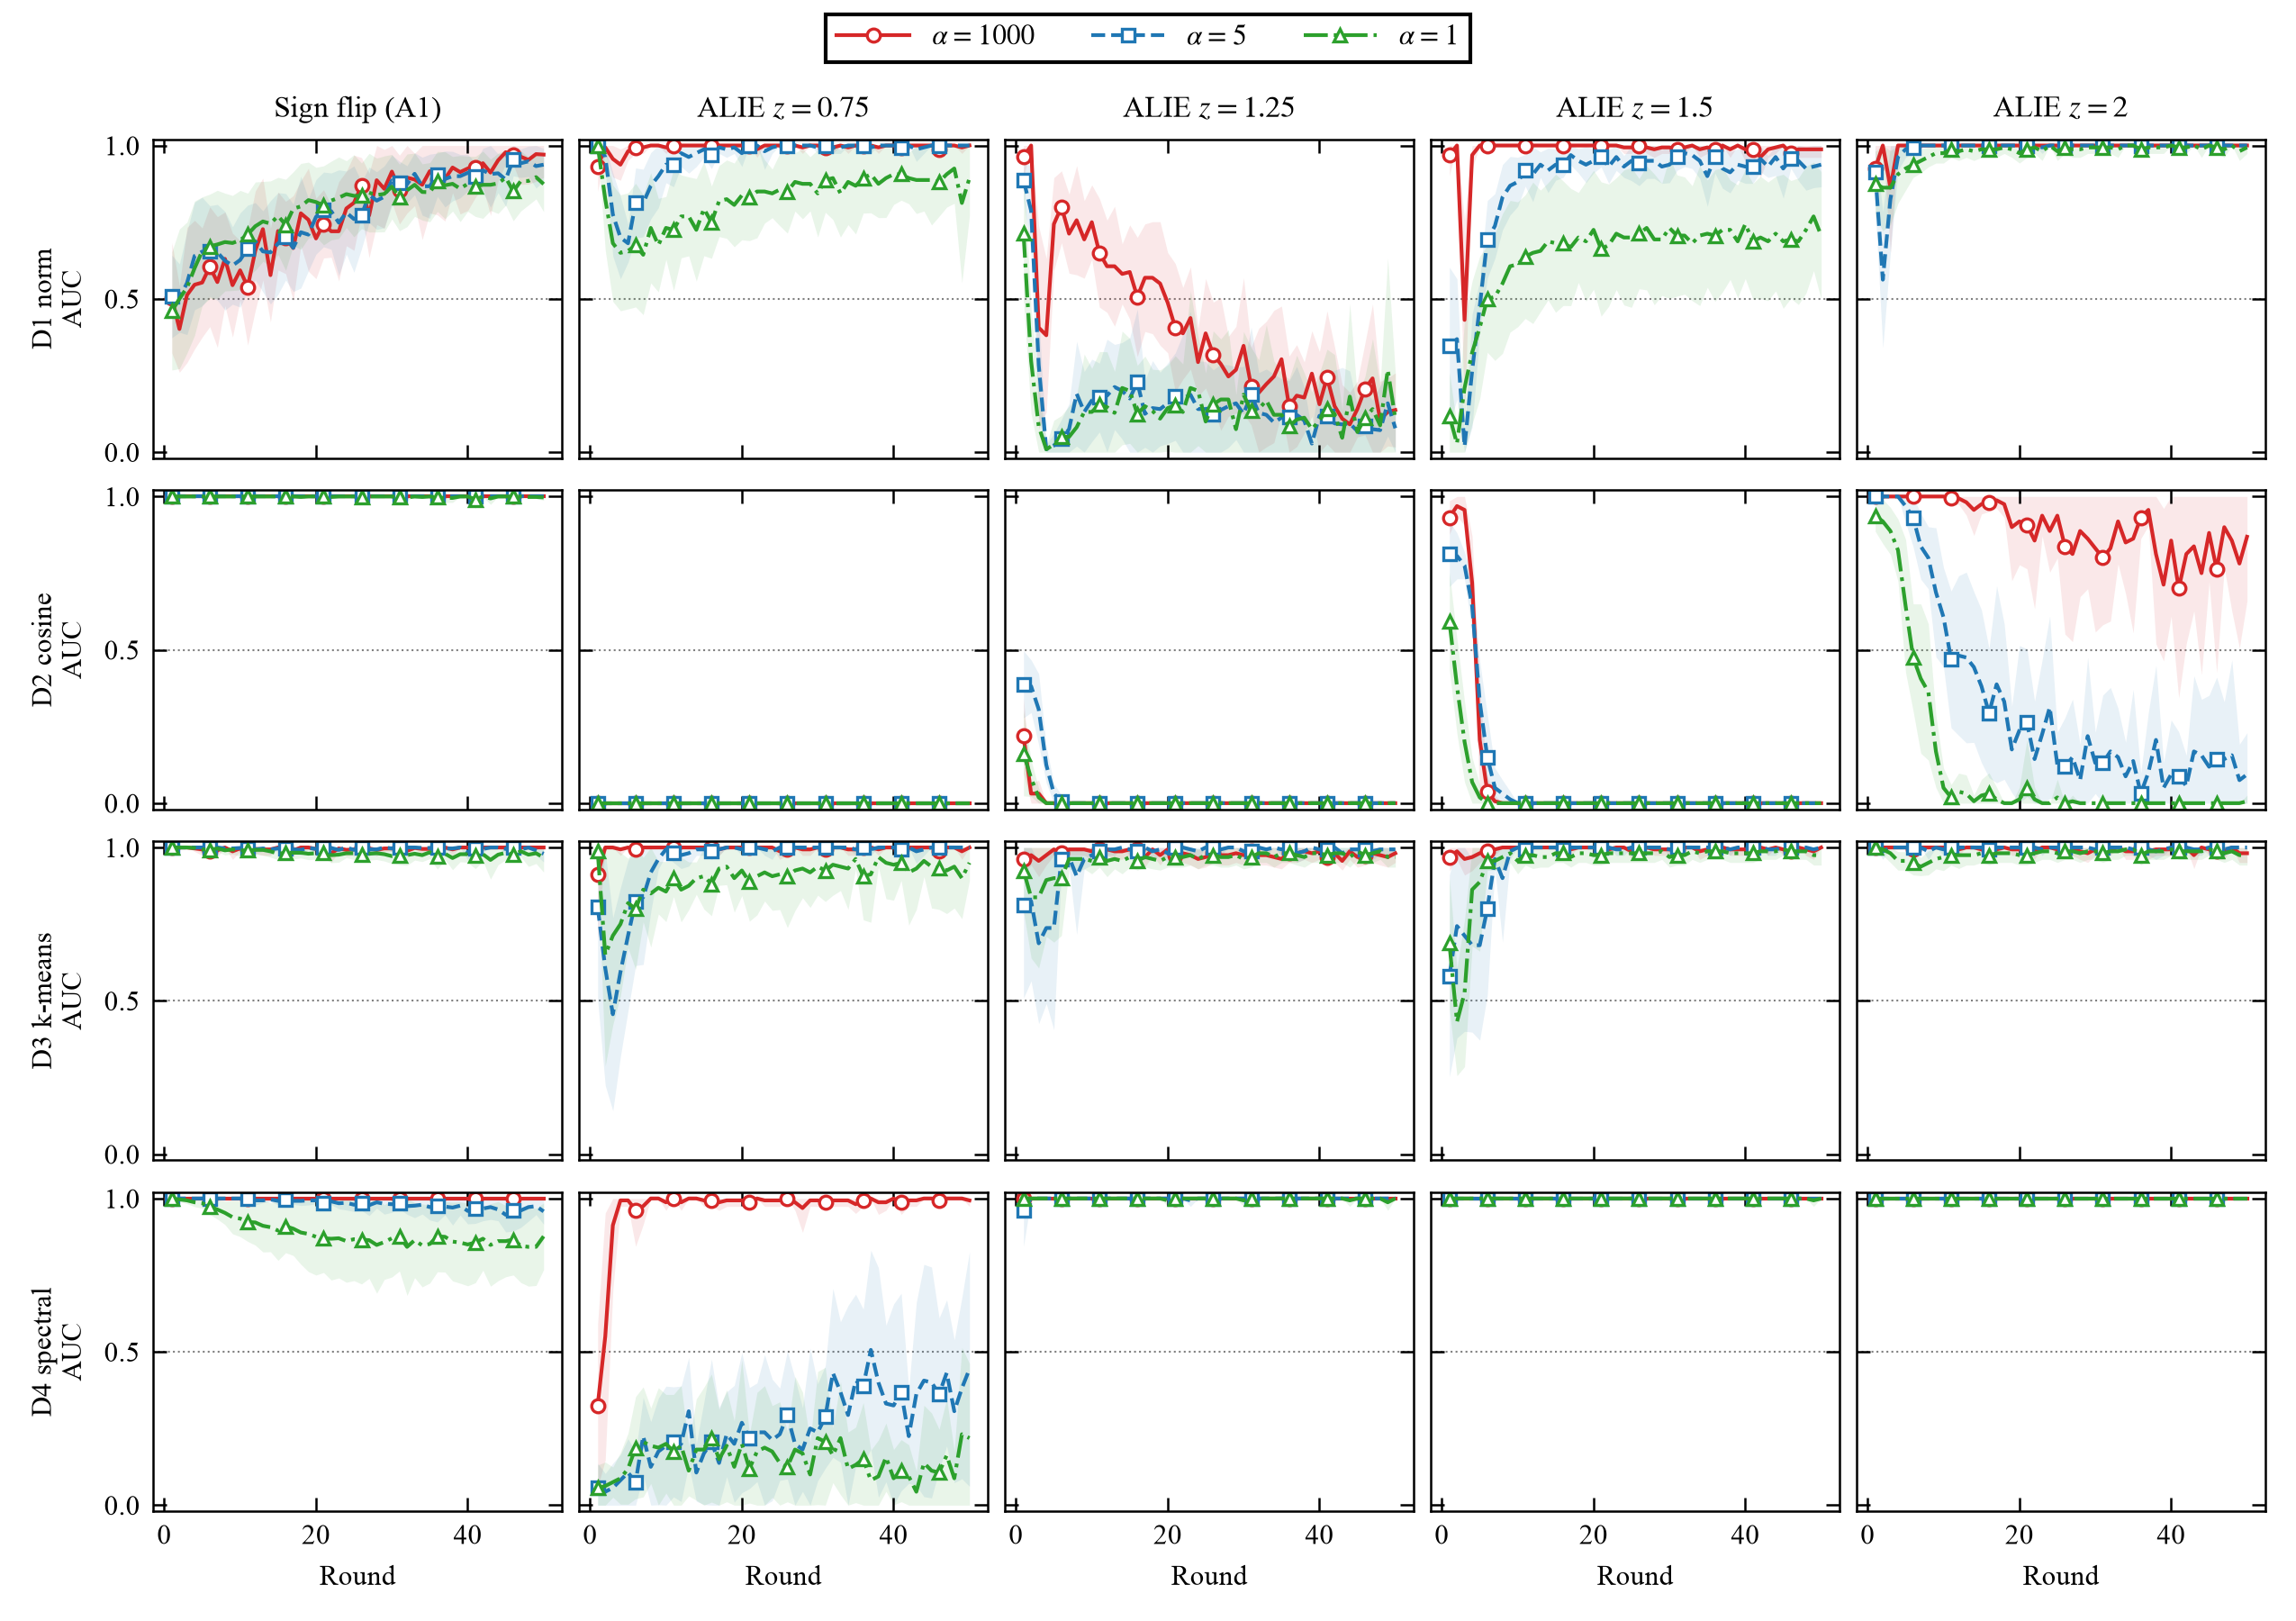
\includegraphics[width=\textwidth]{fig/detection_auc_by_round_v3_sel.png}
\caption{AUC over rounds. Rows are detectors D1--D4 and columns are attacks; for ALIE, four of the eight levels, $z=0.75$, $1.25$, $1.5$, and $2$, are shown (values at rounds 46--50 for the other levels are given in Table~\ref{tab:final-auc} and Fig.~\ref{fig:auc-z}). Lines are means across trials; bands show $\pm$ standard deviation. Red solid line with circles: $\alpha=1000$; blue dashed line with squares: $\alpha=5$; green dash-dotted line with triangles: $\alpha=1$. The dotted line indicates $\mathrm{AUC}=0.5$.}
\label{fig:auc-round}
\end{figure*}

Under sign flipping, D2 stayed at $1.00$ and D3 at $0.97$ or higher in all rounds. In contrast, D1 increased as training progressed for all $\alpha$ (from $0.50$--$0.57$ in rounds 1--5 to $0.87$--$0.93$ in rounds 31--50), and D4 decreased only at $\alpha=1$, from $0.99$ in rounds 1--5 to $0.86$ in rounds 31--50. Thus, detection performance can differ considerably depending on the stage of training, which cannot be seen from the values at rounds 46--50 alone.

\subsection{Non-IID Degree and the Dispersion of Benign Updates}
\label{sec:res-spread}

Table~\ref{tab:spread} shows \Spread{} and the explained variance ratio of the first principal component of benign updates under the no-attack condition.

\begin{table}[t]
\centering
\begin{minipage}[t]{0.52\textwidth}
\centering
\caption{\Spread{} and the explained variance ratio of the first principal component (PC1 ratio) of benign updates under the no-attack condition. ``All rounds'' shows the mean $\pm$ standard deviation of per-round values.}
\label{tab:spread}
\small
\tabcolsep=4.5pt
\begin{tabular}{@{}lcccc@{}}
\toprule
 & \multicolumn{3}{c}{\Spread{}} & PC1 ratio \\
\cmidrule(lr){2-4}\cmidrule(l){5-5}
$\alpha$ & All rounds & Rounds 1--5 & Rounds 46--50 & Rounds 46--50 \\
\midrule
1000 & $0.151 \pm 0.009$ & $0.149$ & $0.143$ & $0.086$ \\
5    & $0.182 \pm 0.070$ & $0.353$ & $0.143$ & $0.122$ \\
1    & $0.211 \pm 0.087$ & $0.434$ & $0.155$ & $0.193$ \\
\bottomrule
\end{tabular}
\end{minipage}\hfill
\begin{minipage}[t]{0.45\textwidth}
\centering
\caption{Spearman's rank correlation coefficient $\rho$ between \PushRatio{} and AUC under the sign-flipping attack (per round; ties handled by average ranks; n/a where AUC is constant and $\rho$ is undefined)}
\label{tab:corr}
\small
\begin{tabular}{@{}lcccc@{}}
\toprule
 & Overall & $\alpha=1000$ & $\alpha=5$ & $\alpha=1$ \\
\midrule
D1 & $-0.17$ & $-0.57$ & $-0.17$ & $\phantom{-}0.69$ \\
D2 & $-0.02$ & n/a & n/a & $\phantom{-}0.06$ \\
D3 & $-0.11$ & $-0.03$ & $\phantom{-}0.07$ & $\phantom{-}0.15$ \\
D4 & $-0.32$ & n/a & $-0.19$ & $-0.12$ \\
\bottomrule
\end{tabular}
\end{minipage}
\end{table}

In rounds 1--5, \Spread{} for $\alpha=5,\,1$ was $0.353$ and $0.434$, about $2.4$--$2.9$ times the $0.149$ of $\alpha=1000$, whereas in rounds 46--50 the ratio was only $1.00$--$1.08$. On the other hand, the explained variance ratio of the first principal component still differed by a factor of about $2.2$ in rounds 46--50: $0.086$, $0.122$, and $0.193$ for $\alpha=1000,\,5,\,1$.

Under the attacked conditions, the mean \PushRatio{} over rounds 46--50 was $1.00$--$1.02$ times $z$ for ALIE regardless of $\alpha$, and $1.5$ or higher for all $\alpha$ under sign flipping.

For ALIE, $|\cos\theta|$ between the malicious direction and the first principal component of all updates corresponded well with D4's AUC ($\rho=0.92$ over 24 conditions). For example, at $z=0.75$, $|\cos\theta|$ was $0.920$, $0.305$, and $0.138$ for $\alpha=1000,\,5,\,1$, corresponding to D4's AUC ($0.998$, $0.385$, $0.161$). The explained variance ratio of the first principal component of benign updates under these attacked conditions was $0.102$, $0.141$, and $0.207$.

\subsection{Relationship between \PushRatio{} and AUC under the Sign-Flipping Attack}
\label{sec:res-pushratio}

For the sign-flipping attack, Table~\ref{tab:corr} shows Spearman's rank correlation coefficient $\rho$ between \PushRatio{} and AUC. Each round of each run is treated as one point, and the correlation is computed for each detector overall ($1{,}500$ points) and for each $\alpha$ ($500$ points each).

The rank correlation between the two was weak or negative both overall and for each $\alpha$, with the only exception being D1 at $\alpha=1$ ($\rho=0.69$).

\section{Discussion}
\label{sec:discussion}

\subsection{Differences among Detectors}
\label{sec:disc-detectors}

Against the sign-flipping attack, D2 and D3 showed high detection performance for all $\alpha$ (Table~\ref{tab:final-auc}). This is likely because benign updates share a common direction. Letting $\theta$ be the angle between a benign update $g$ and the reference direction $r$, the D2 score is $1-\cos\theta$ for the benign update and $1+\cos\theta$ for the sign-flipped malicious update. Hence, as long as $\cos\theta>0$, the two are always separated in ranking. Indeed, the mean scores in rounds 1--5 at $\alpha=1000$ were $0.04$ for benign updates and $1.95$ for malicious updates (Fig.~\ref{fig:signflip-d2}). D3 also includes the D2 score as a feature, and $|\cos|$ between the malicious direction and the first principal component of all updates was $0.96$ or higher for all $\alpha$, so it is easily separated by the same property. However, as training progressed, benign updates became less aligned and both scores approached $1$ ($0.74$ for benign updates and $1.16$ for malicious updates in rounds 46--50 at $\alpha=1000$).

\begin{figure}[t]
\centering
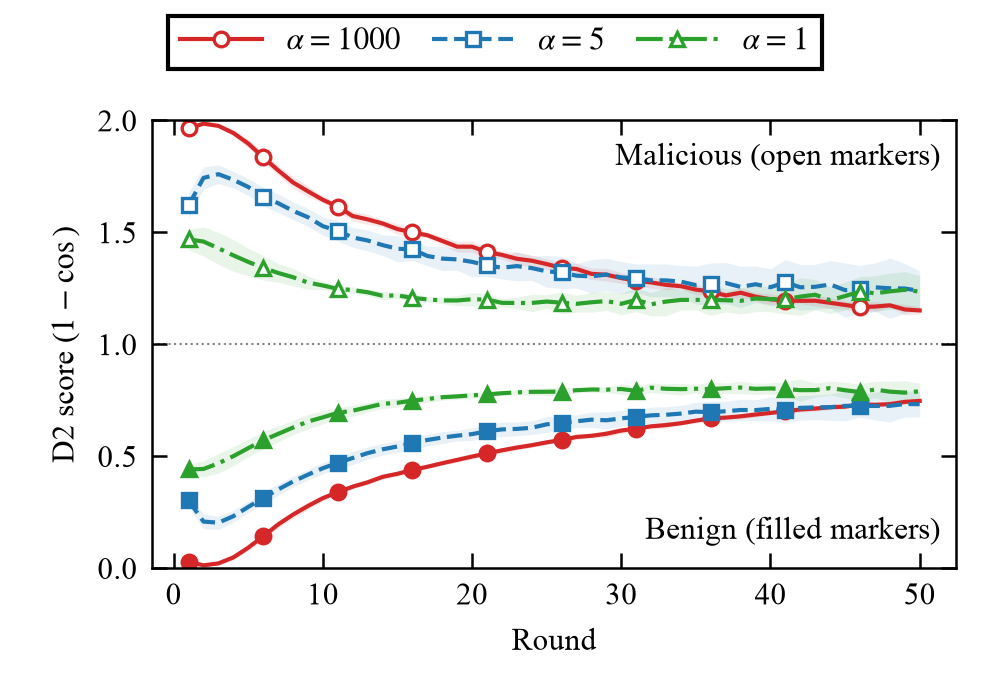
\includegraphics[width=0.5\textwidth]{fig/signflip_d2_score_by_round_v3.png}
\caption{D2 score (cosine distance to the reference direction) over rounds under the sign-flipping attack. Open markers show the mean of malicious updates and filled markers the mean of benign updates (mean over 10 trials; bands show $\pm$ standard deviation). Red solid line with circles: $\alpha=1000$; blue dashed line with squares: $\alpha=5$; green dash-dotted line with triangles: $\alpha=1$. The dotted line indicates score $1$, corresponding to $\cos\theta=0$.}
\label{fig:signflip-d2}
\end{figure}

Against ALIE, D2's AUC was $0.00$ under all conditions with $z \le 1.5$ (Table~\ref{tab:final-auc}). This means that every malicious update was judged more benign than every benign update, i.e., the ranking was completely inverted. D2's reference direction $r$ is the coordinate-wise median of all updates; since the four malicious updates are all the same vector and lie on the same side below the mean in every coordinate, $r$ is pulled toward the malicious updates. In contrast, the deviations of individual benign clients point in different directions coordinate by coordinate, and in high dimensions they are nearly orthogonal to the malicious direction. As a result, the D2 scores of benign updates were nearly $1$, exceeding the scores of malicious updates ($0.22$--$0.33$ at $z=1$).

D3 achieved AUC of $0.92$ or higher against ALIE under all conditions. D3's score is the distance from the centroid of the benign cluster, which grows regardless of the direction of deviation, so it also detects the kind of deviation that caused the ranking inversion in D2. In addition, since the four malicious clients send an identical vector under ALIE, the malicious updates coincide at a single point in feature space and are easily separated.

From the above, the first question can be answered as follows. The ranking of detectors switches depending on the attack, and the success of detection is determined by the combination of two factors: where the attack places malicious updates, and which quantity a detector looks at and which direction of deviation it regards as anomalous.

\subsection{Effect of Non-IID Degree on Detection Performance}
\label{sec:disc-noniid}

Non-IID data degraded detection performance, but this degradation cannot be explained by the increase in the dispersion of benign updates \Spread{} predicted by the central hypothesis. \Spread{} was larger for smaller $\alpha$ early in training (about $2.4$--$2.9$ times that of $\alpha=1000$ in rounds 1--5), but in rounds 46--50 the ratio was $1.00$--$1.08$, showing almost no difference (Table~\ref{tab:spread}). Meanwhile, detection performance differed substantially across $\alpha$ mainly in the latter half of training.

What instead corresponded to the degradation in detection performance was how the dispersion was distributed. First, Non-IID data increased the variation in the norms of benign updates (the coefficient of variation in rounds 46--50 under sign flipping was $0.08$, $0.17$, and $0.39$ for $\alpha=1000,\,5,\,1$), degrading the detection performance of the norm-dependent D1 and D4 against sign flipping. Second, because Non-IID data points each client's update in a different direction, the common component becomes small relative to each client's deviation, which increased the $z$ at which D2 begins to detect ALIE ($z=2$ at $\alpha=1000$ and $z=3$ at $\alpha=1$). Third, Non-IID data concentrated the dispersion of benign updates in a particular direction. For ALIE at $z=0.75$, although \PushRatio{} was about $0.75$ for every $\alpha$, D4's AUC was $1.00$, $0.39$, and $0.16$ for $\alpha=1000,\,5,\,1$, and was lower the larger the explained variance ratio of the first principal component of benign updates ($0.102$, $0.141$, $0.207$; Section~\ref{sec:res-spread}).

From the above, the second question can be answered as follows. Non-IID data degrades detection performance, but the degradation cannot be explained by an increase in \Spread{}; it corresponded instead to how the dispersion was distributed. Li et al.\ (2023)\cite{li2023experimental} reported that Non-IID data reduces the robustness of several Robust Aggregation methods in terms of final accuracy. Our results are consistent with this, and complement the results of Li et al.\ (2023) by evaluating the same phenomenon from the viewpoint of detection performance and showing that the degradation corresponds to the shape of the distribution of benign updates.

\subsection{Attack Stealthiness and the Boundary of Detection Breakdown}
\label{sec:disc-rq3}

The central hypothesis predicted that detection performance drops sharply once \PushRatio{} falls below $1$. Since $\PushRatio \approx z$ for ALIE, the levels with $z<1$ correspond to this region. However, even at the innermost level $z=0.385$, D1 and D3 detected malicious updates with AUC of $0.96$ or higher for all $\alpha$ (Table~\ref{tab:final-auc}).

This result can be explained by the arrangement of benign updates in high-dimensional space. The squared distance of a benign update from the mean is a sum of about 260,000 positive values, so it is expected to concentrate around nearly the same value across benign updates. Indeed, the coefficient of variation of the distance of benign updates from the mean in rounds 46--50 was about $0.08$, $0.09$, and $0.18$ for $\alpha=1000,\,5,\,1$. That is, benign updates lie on a thin shell at an almost constant distance from the mean, and there are almost none near the mean. Therefore, the malicious update at $z=0.385$ lies inside the shell and is distinguished from benign updates precisely because it is too close to the mean. Note, however, that this interpretation was formulated after seeing the results.

\begin{figure*}[t]
\centering
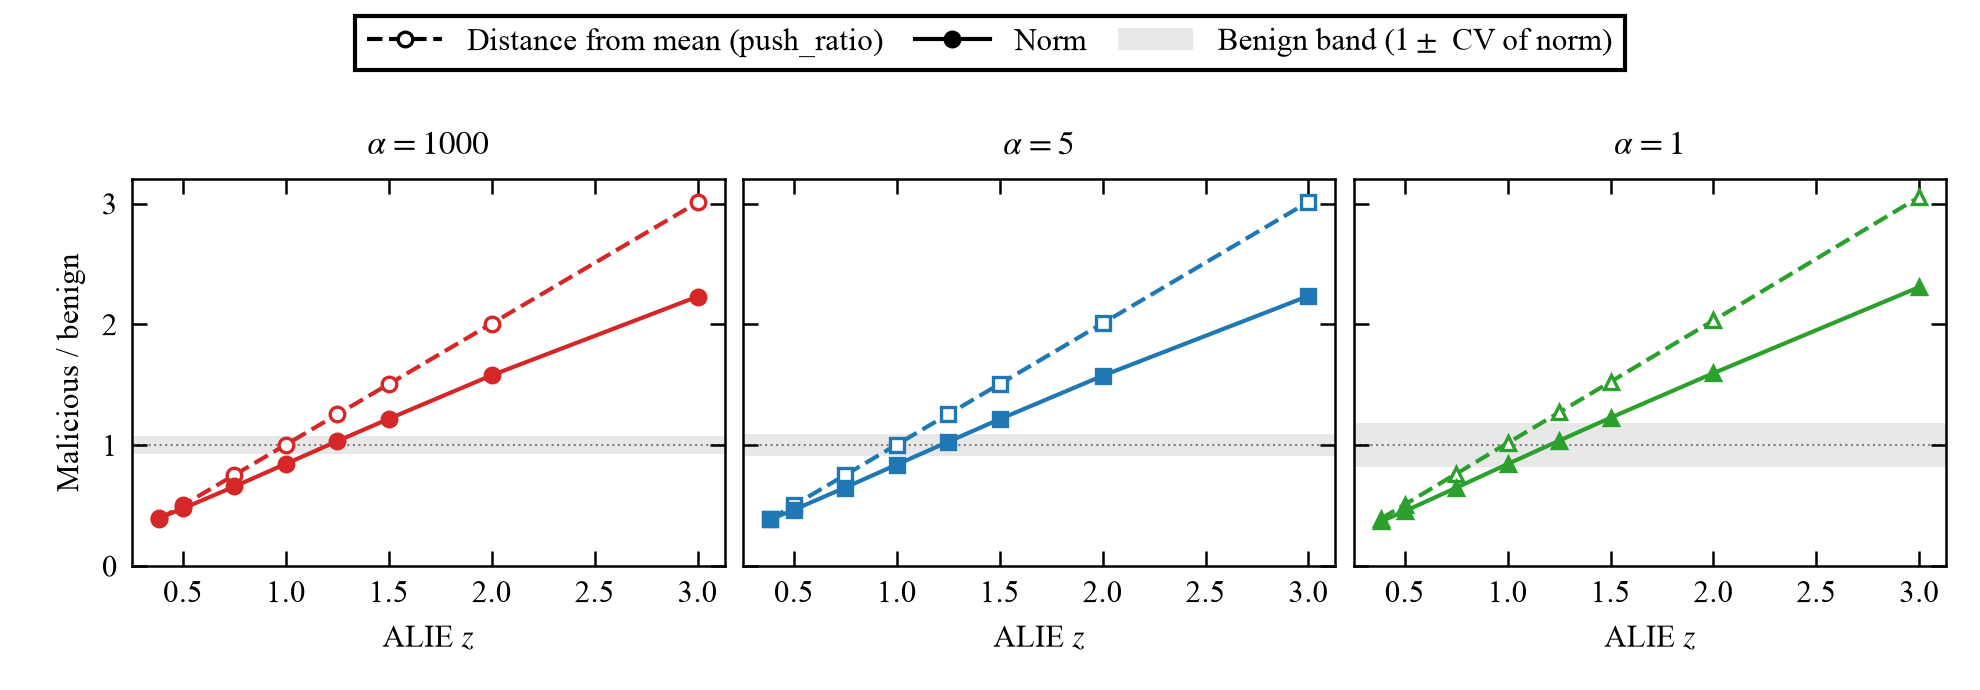
\includegraphics[width=0.85\textwidth]{fig/alie_shell_by_z_v3.png}
\caption{ALIE's $z$ and the ratio of malicious updates to benign updates (rounds 46--50, mean over 10 trials). Dashed lines (open markers) show the ratio of distances from the mean (\PushRatio{}), and solid lines (filled markers) show the norm ratio. The gray band is $1 \pm$ the coefficient of variation of benign update norms, indicating the approximate thickness of the shell of benign updates. The dotted line indicates a ratio of $1$.}
\label{fig:alie-shell}
\end{figure*}

As $z$ increases, the malicious update approaches the shell, and with even larger $z$ it moves outside the shell (Fig.~\ref{fig:alie-shell}). Hence, detection based on distance or norm is most difficult around the point where the malicious update lies on the shell. Indeed, D1's AUC was minimized for all $\alpha$ ($0.09$--$0.16$) at $z=1.25$, where the norm of malicious updates matches that of benign updates, and returned to $0.99$ or higher for $z \ge 2$.

From the above, the third question can be answered as follows. Moving malicious updates closer to the mean of benign updates is not a means of evading detection. $\PushRatio=1$ is not the boundary at which detection breaks down, but is near the point where malicious updates lie on the shell and are best hidden from distance- or norm-based detection.

\subsection{Evaluation of the Central Hypothesis}
\label{sec:disc-hyp}

The central hypothesis consists of three claims: (1) Non-IID data increases \Spread{}; (2) detectability is largely determined by \PushRatio{}, and detection performance drops sharply once it falls below $1$; and (3) consequently, Non-IID data degrades detection performance. Claim (1) held early in training but hardly held once training had progressed (Section~\ref{sec:disc-noniid}). Claim (2) was not supported. Under sign flipping, the overall rank correlation between \PushRatio{} and AUC was between $-0.32$ and $-0.02$, with no positive correlation observed (Table~\ref{tab:corr}). Moreover, for ALIE, detection performance did not drop sharply even for $z<1$ (Section~\ref{sec:disc-rq3}), and at $z=0.75$ D4's AUC differed greatly across $\alpha$ despite the same \PushRatio{} (Section~\ref{sec:disc-noniid}). Claim (3) was observed, but the reason was not an increase in \Spread{} but how the dispersion was distributed.

We consider two main reasons why the hypothesis failed. First, the central hypothesis was based on the low-dimensional intuition that benign updates fill the region around their mean. In reality, high-dimensional benign updates lie on a shell at an almost constant distance from the mean, so malicious updates close to the mean were in fact conspicuous. Second, \PushRatio{} summarizes the position of malicious updates in a single quantity, ``the distance from the benign mean,'' whereas each detector looks at a different quantity and regards a different direction of deviation as anomalous. Therefore, explaining detectability requires considering where malicious updates lie in the quantity each detector looks at, and the shape of the distribution of benign updates.

Note that most ALIE settings in this study hardly reduced accuracy under FedAvg, so our results mainly concern detection performance. In addition, the experiments were conducted under limited conditions: MNIST, 20 clients, and Non-IID data limited to label skew.

\section{Conclusion}
\label{sec:conclusion}

In this study, we evaluated the detectability of malicious updates in FL from two viewpoints, the degree of data heterogeneity (Non-IID degree) and the stealthiness of the attack, using the ROC-AUC of four detectors. The results showed that whether detection succeeds is determined by where malicious updates lie in the quantity a detector looks at, and which direction of deviation the detector regards as anomalous. Non-IID data degraded detection performance, but the cause was not the magnitude of the dispersion of benign updates but how that dispersion was distributed. Consequently, the central hypothesis that detectability is largely determined by the ratio between the push of malicious updates and the dispersion of benign updates was not supported.

{\small
\begin{thebibliography}{99}

\bibitem{mammen2021fl}
Priyanka Mary Mammen,
``Federated Learning: Opportunities and Challenges,''
arXiv preprint arXiv:2101.05428, 2021.

\bibitem{sagar2023survey}
Subhash Sagar, Chang-Tsun Li, Seng W. Loke, Jinho Choi,
``Poisoning Attacks and Defenses in Federated Learning: A Survey,''
arXiv preprint arXiv:2301.05795, 2023.

\bibitem{baruch2019little}
Gilad Baruch, Moran Baruch, Yoav Goldberg,
``A Little Is Enough: Circumventing Defenses For Distributed Learning,''
Advances in Neural Information Processing Systems (NeurIPS), 2019.

\bibitem{li2023experimental}
Shenghui Li, Edith C.-H. Ngai, Thiemo Voigt,
``An Experimental Study of Byzantine-Robust Aggregation Schemes in Federated Learning,''
arXiv preprint arXiv:2302.07173, 2023.

\bibitem{fang2020local}
Minghong Fang, Xiaoyu Cao, Jinyuan Jia, Neil Zhenqiang Gong,
``Local Model Poisoning Attacks to Byzantine-Robust Federated Learning,''
Proceedings of the 29th USENIX Security Symposium (USENIX Security 2020),
pp.~1605--1622, 2020.

\bibitem{blanchard2017krum}
Peva Blanchard, El Mahdi El Mhamdi, Rachid Guerraoui, Julien Stainer,
``Machine Learning with Adversaries: Byzantine Tolerant Gradient Descent,''
Advances in Neural Information Processing Systems (NeurIPS), 2017.

\bibitem{yin2018byzantine}
Dong Yin, Yudong Chen, Kannan Ramchandran, Peter Bartlett,
``Byzantine-Robust Distributed Learning: Towards Optimal Statistical Rates,''
Proceedings of the 35th International Conference on Machine Learning (ICML), 2018.

\bibitem{elmhamdi2018hidden}
El Mahdi El Mhamdi, Rachid Guerraoui, S\'ebastien Rouault,
``The Hidden Vulnerability of Distributed Learning in Byzantium,''
Proceedings of the 35th International Conference on Machine Learning (ICML), 2018.

\bibitem{shejwalkar2021manipulating}
Virat Shejwalkar, Amir Houmansadr,
``Manipulating the Byzantine: Optimizing Model Poisoning Attacks and Defenses for Federated Learning,''
Network and Distributed System Security Symposium (NDSS), 2021.

\bibitem{nguyen2022flame}
Thien Duc Nguyen et al.,
``FLAME: Taming Backdoors in Federated Learning,''
31st USENIX Security Symposium (USENIX Security 2022), pp.~1415--1432, 2022.

\bibitem{hsu2019measuring}
Tzu-Ming Harry Hsu, Hang Qi, Matthew Brown,
``Measuring the Effects of Non-Identical Data Distribution for Federated Visual Classification,''
arXiv preprint arXiv:1909.06335, 2019.

\bibitem{li2022federated}
Qinbin Li, Yiqun Diao, Quan Chen, Bingsheng He,
``Federated Learning on Non-IID Data Silos: An Experimental Study,''
Proceedings of the 38th IEEE International Conference on Data Engineering (ICDE), 2022.

\bibitem{wang2023trust}
Zhilin Wang, Qin Hu, Xukai Zou,
``Can We Trust the Similarity Measurement in Federated Learning?,''
arXiv preprint arXiv:2311.03369, 2023.

\bibitem{cao2021fltrust}
Xiaoyu Cao, Minghong Fang, Jia Liu, Neil Zhenqiang Gong,
``FLTrust: Byzantine-robust Federated Learning via Trust Bootstrapping,''
Network and Distributed System Security Symposium (NDSS), 2021.

\bibitem{shejwalkar2022back}
Virat Shejwalkar, Amir Houmansadr, Peter Kairouz, Daniel Ramage,
``Back to the Drawing Board: A Critical Evaluation of Poisoning Attacks on Production Federated Learning,''
IEEE Symposium on Security and Privacy (S\&P), 2022.

\bibitem{mcmahan2017fedavg}
H.~Brendan McMahan, Eider Moore, Daniel Ramage, Seth Hampson, Blaise Aguera y Arcas,
``Communication-Efficient Learning of Deep Networks from Decentralized Data,''
Proceedings of the 20th International Conference on Artificial Intelligence and Statistics (AISTATS),
pp.~1273--1282, 2017.

\bibitem{shen2016auror}
Shiqi Shen, Shruti Tople, Prateek Saxena,
``Auror: Defending Against Poisoning Attacks in Collaborative Deep Learning Systems,''
Proceedings of the 32nd Annual Conference on Computer Security Applications (ACSAC), 2016.

\bibitem{tran2018spectral}
Brandon Tran, Jerry Li, Aleksander Madry,
``Spectral Signatures in Backdoor Attacks,''
Advances in Neural Information Processing Systems (NeurIPS), 2018.

\bibitem{fawcett2006roc}
Tom Fawcett,
``An Introduction to ROC Analysis,''
Pattern Recognition Letters, vol.~27, no.~8, pp.~861--874, 2006.

\bibitem{hanley1982meaning}
James A. Hanley, Barbara J. McNeil,
``The Meaning and Use of the Area under a Receiver Operating Characteristic (ROC) Curve,''
Radiology, vol.~143, no.~1, pp.~29--36, 1982.

\bibitem{beutel2020flower}
Daniel J. Beutel, Taner Topal, Akhil Mathur, Xinchi Qiu, Javier Fernandez-Marques, Yan Gao, Lorenzo Sani, Kwing Hei Li, Titouan Parcollet, Pedro Porto Buarque de Gusm\~{a}o, Nicholas D. Lane,
``Flower: A Friendly Federated Learning Research Framework,''
arXiv preprint arXiv:2007.14390, 2020.

\end{thebibliography}
}

\end{document}
